\documentclass{article}
\usepackage{amsmath}
\usepackage{amssymb}
\usepackage{graphicx}
\usepackage{hyperref}
\usepackage[version=4]{mhchem}


\begin{document}
In right triangle \(A B C, M\) and \(N\) are midpoints of legs \(\overline{A B}\) and \(\overline{B C}\), respectively. Leg \(\overline{A B}\) is 6 units long, and leg \(\overline{B C}\) is 8 units long. How many square units are in the area of \(\triangle A P C\) ? (Mathcounts Competitions)

Solution: 8 (square units)\\
\centering
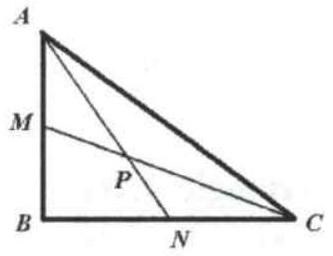
\includegraphics[width=\textwidth]{images/009(1).jpg}

We draw the third median \(B D\).

These three medians divide the triangle into six equal areas. The area of triangle \(A B C\) is \(6 \times 8 / 2=24\).\\
The area of \(\triangle A P C\) is just \(\frac{2}{6} \times 24=8\).\\
\centering
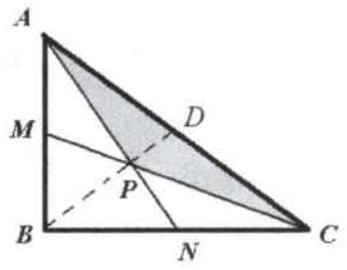
\includegraphics[width=\textwidth]{images/009.jpg}


\end{document}
